{
After selecting the convenient features for each of the 
physical parameters we are interested in, the next step will be
to produce the effective model becoming useful to predict those 
parameters. In order to do that, the noised, theoretical 
BT-Settl library was used again by splitting-out 33\% as for testing 
and using the remaining 66\% for training.
In order to produce reslient models, a ten folders 
crossvalidation without repetition was adopted, where the best 
model in the training folders was retained as the 
most convenient.
}

\subsection{Models considered.}
\label {ssub:models}
{
As a classical regression problem several linear and non-linear
modelling techniques with specific research for 
adequate parameters per method when required, were considered:
\begin{itemize}
 \item {Generalized Linear Models (GLM).}
 \item {Generalized Additive Models (GAM).}
 \item {Project Pursuit Regression Method (PPR).}
 \item {Ridge Regression Model (RRM).}
 \item {Kernel Partial Least Square Method (KPLS).}
 \item {Multiadaptative Spline Regression Models (MARS).}
 \item {Random Forest Regression Models (RF).}
 \item {Gradient Boosting with Regression Trees (GBR).}
 \item {Generalized Boosted Regression Models (GBM).}
 \item {Support Vector Machine Models with Gaussian Kernel (SVM).}
 \item {MLP Nerural Networks (NNET).}
\end{itemize}

We have considered, in addition to the previous models, 
two ensembles techniques among the already built models, 
one linear and another one Greedy; 
all these models were considered in order to produce 
the most suitable model to be brought as predictor.
}

{
Comparison of performance between sets of features for temperature 
can be analyzed, over the same testing subdataset and it was depicted 
in Table~\ref{tab:model_TSD}.

\begin{table}
\begin{center}
\begin{tabular}{rrrrrrr}
  \hline
  SNR & Features & SVM & RF & GLM  & MARS & Greedy \\
  \hline
  \multirow{2}{*}{50}  &  Cesetti et al. & 81.6 &  83.3 & 163.5 & 91.9 & 71.4 \\
      &  GA             & 91.4 & 82.2 & 161.1  & 91.9 & 77.3 \\
  \multirow{2}{*}{10}  &  Cesetti et al. & 135.8 & 138.5 & 268.8 & 166.8 & 125.9 \\
      &  GA             & 123.2 & 122.6 & 212.6 & 130.9 & 116.5 \\
   \hline
\end{tabular}
\caption { RSME for different models predicting $T_{eff}$ [K].} 
\label{tab:model_TSD} 
\end{center}
\end{table}

After calculating the bartlett test for both cases of SNR it was 
seen that variances are homogeneous since p > 0.05, and 
the Flinger-Killen shows that homkedascity is verified, 
then F-ANOVA test makes clear that there is no significative 
difference between models. Then, it is possible to conclude
that quality of features from both sources are equivalent
regarding modeling capability, even when GA only has proposed five
features and Cesetti et al. requires seven features.

}

\subsection{Full Spectra Oriented Models}
\label {ssub:GM_BPG}
{
As an alternative to build modles based on bandpasses, 
a similiar methodology to the one depicted in (\cite{2013A&A...550A.120S})
was implemented.

For the projection an Independend Component Analysis (ICA) with ten dimensions
was used and for Temperature regression an optimized SVM 
with parameters of C=10 and $\epsilon$=0.001.

Considering the Gravity case, the most suitable ICA had twentysix dimensions and the 
best SVM parameters were C=1000 and $\epsilon = 0.001 $. This was the same case
for Metallicity.

In terms of interpretation, this methodology looks to predict the physical paramenters
by considering the whole star spectrum instead of information provided 
by specific bands. Thus it can be interesting to analyze suitability 
for prediction against the other approach.

In the same sense it was decided to consider direct selection, which is
also a technique based on the whole espectrum but, instead of regressing
specific parameters, the closest labeled spectrum to the one 
under analysis is identified by a $\chi^2$ distance.
This becomes possible as interpolation between labeled spectra can be
easily performed.

}

\subsection{Temperature model based on Spectral Subtyoe.}
\label {ssub:TLSB}
{
% Luis ¿esto lo explicas tu?
}

\subsection{Temperature Model for $T_{eff}$.}
\label {ssub:teff_model}
{
After training the set of models by using labelled BT-Settl dataset, those models 
were used to predict the IPAC temperature.
In Figure~\ref{fig:t50ga_tsb} the relationship between Temperature estimated from 
GA proposed features with SNR=50 and the Temperature estimation 
from spectral subtype.

\begin {figure}
 \begin{center}
 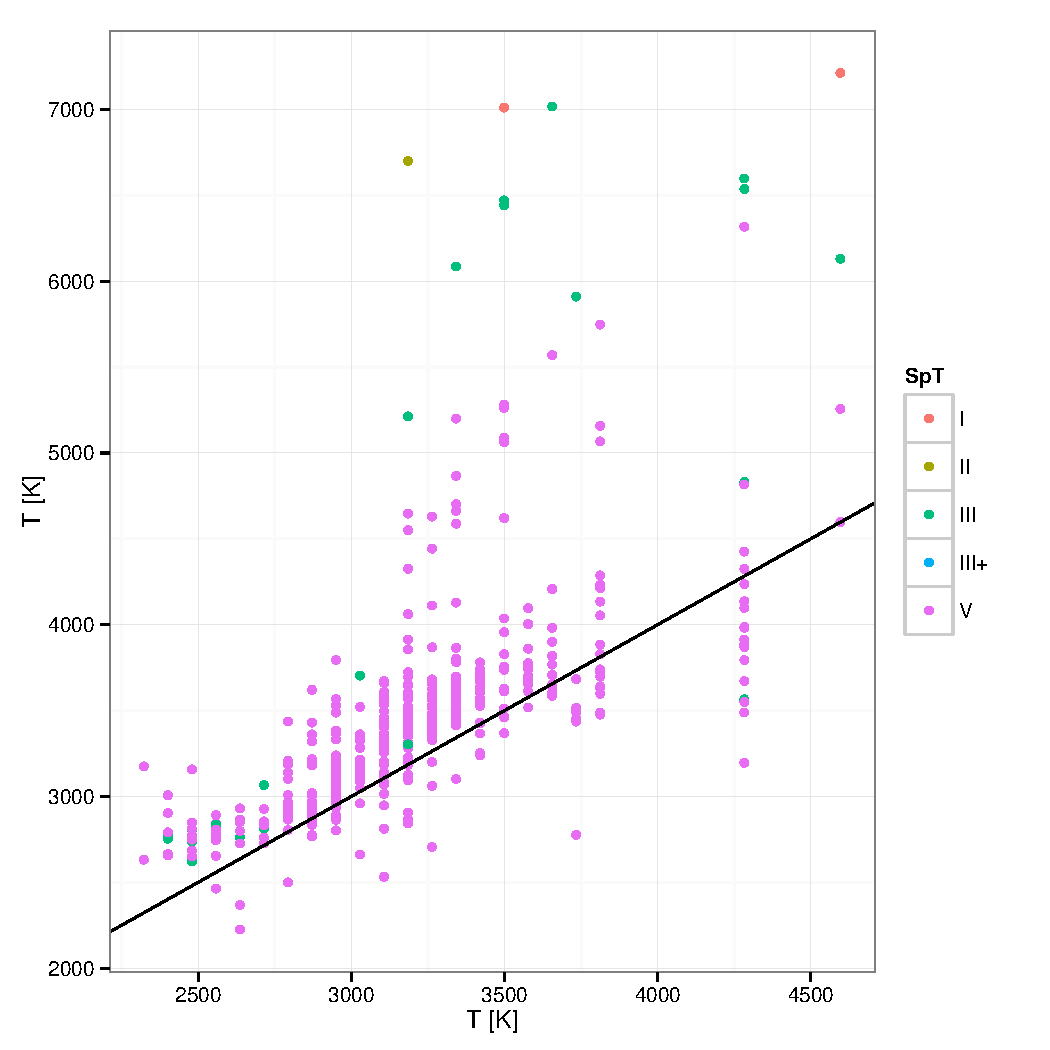
\includegraphics[width=6cm]{figs/T50GA_TSB.pdf}
 \caption{Comparison between Temperature estimations from Spectral Subtype 
 in x axis and the Random Forest for Ga based features trained with BT-Settl 
 at SNR=50 on y-axis}
 \label{fig:t50ga_tsb}
 \end{center}
\end {figure}

Similarly Figure~\ref{fig:t10ga_tsb} shows the relationship against GA features 
and Random Forest model trained by BT-Settl at SNR=10.
\begin {figure}
 \begin{center}
 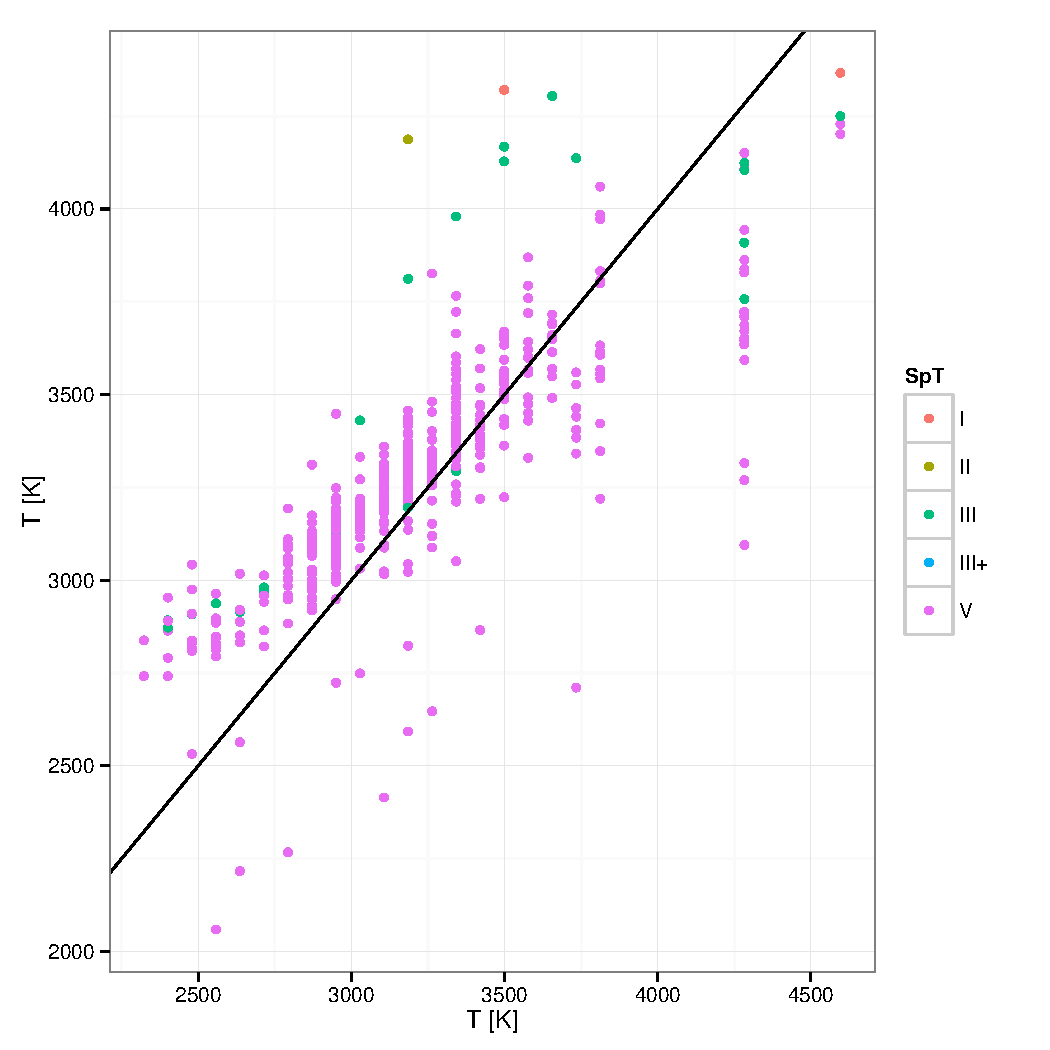
\includegraphics[width=6cm]{figs/T10GA_TSB.pdf}
 \caption{Comparison between Temperature estimations from Spectral Subtype 
 in x axis and the Random Forest for Ga based features trained with BT-Settl 
 at SNR=10 on y-axis}
 \label{fig:t10ga_tsb}
 \end{center}
\end {figure}

The same was made with features forposed by Cesetti et al. 
(see Figure~\ref{fig:t50cs_tsb} and Figure~\ref{fig:t10cs_tsb}).

\begin {figure}
 \begin{center}
 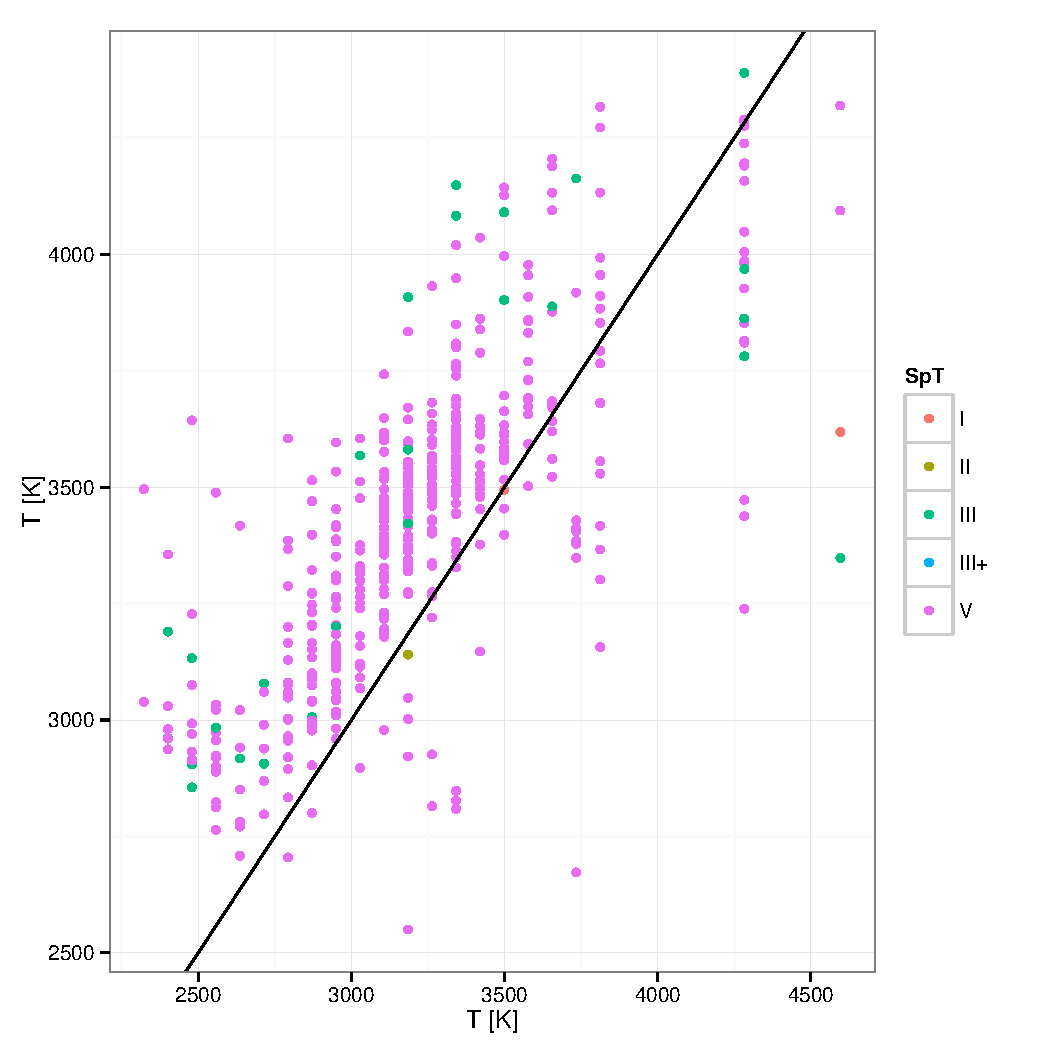
\includegraphics[width=6cm]{figs/T50CS_TSB.pdf}
 \caption{Comparison between Temperature estimations from Spectral Subtype 
 in x axis and the Random Forest for Cesetti et al. features trained with BT-Settl 
 at SNR=50 on y-axis}
 \label{fig:t50cs_tsb}
 \end{center}
\end {figure}

\begin {figure}
 \begin{center}
 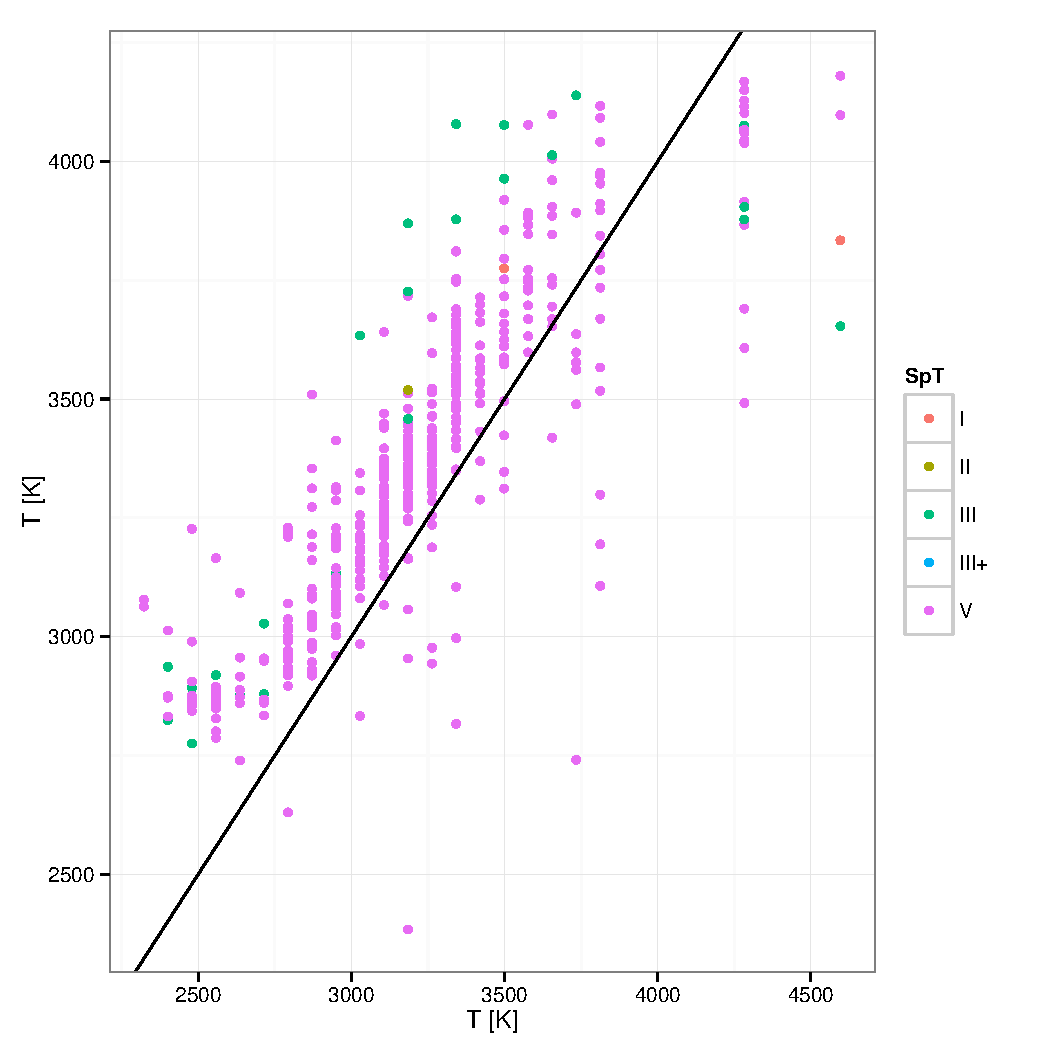
\includegraphics[width=6cm]{figs/T10CS_TSB.pdf}
 \caption{Comparison between Temperature estimations from Spectral Subtype 
 in x axis and the Random Forest for Cesetti et al. features trained with BT-Settl 
 at SNR=10 on y-axis}
 \label{fig:t10cs_tsb}
 \end{center}
\end {figure}

The analysis was done for Global spectrum based approach. 
Thus in Figure~\ref{fig:t50bp_tsb} and Figure~\ref{fig:t10bp_tsb} presents the relationship for 
the diemensional reduction and SVM approach and 
Figure~\ref{} and Figure~\ref{} accounts for similarity 
based estimation of pysical parameters accoding to $\chi^2$ metric.

\begin {figure}
 \begin{center}
 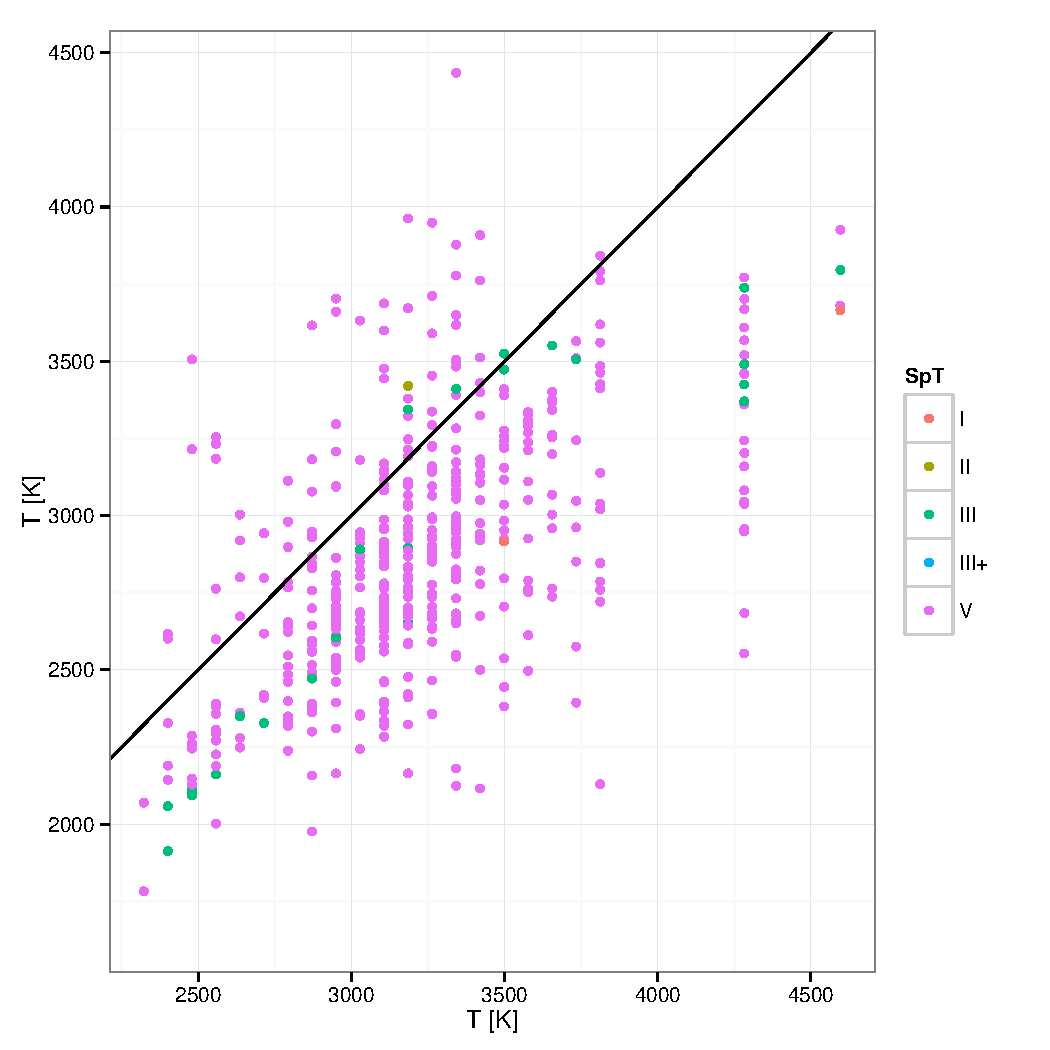
\includegraphics[width=6cm]{figs/T50BP_TSB.pdf}
 \caption{Comparison between Temperature estimations from Spectral Subtype 
 in x axis and the Random Forest for full length spectra trained with BT-Settl 
 at SNR=50 on y-axis}
 \label{fig:t50bp_tsb}
 \end{center}
\end {figure}

\begin {figure}
 \begin{center}
 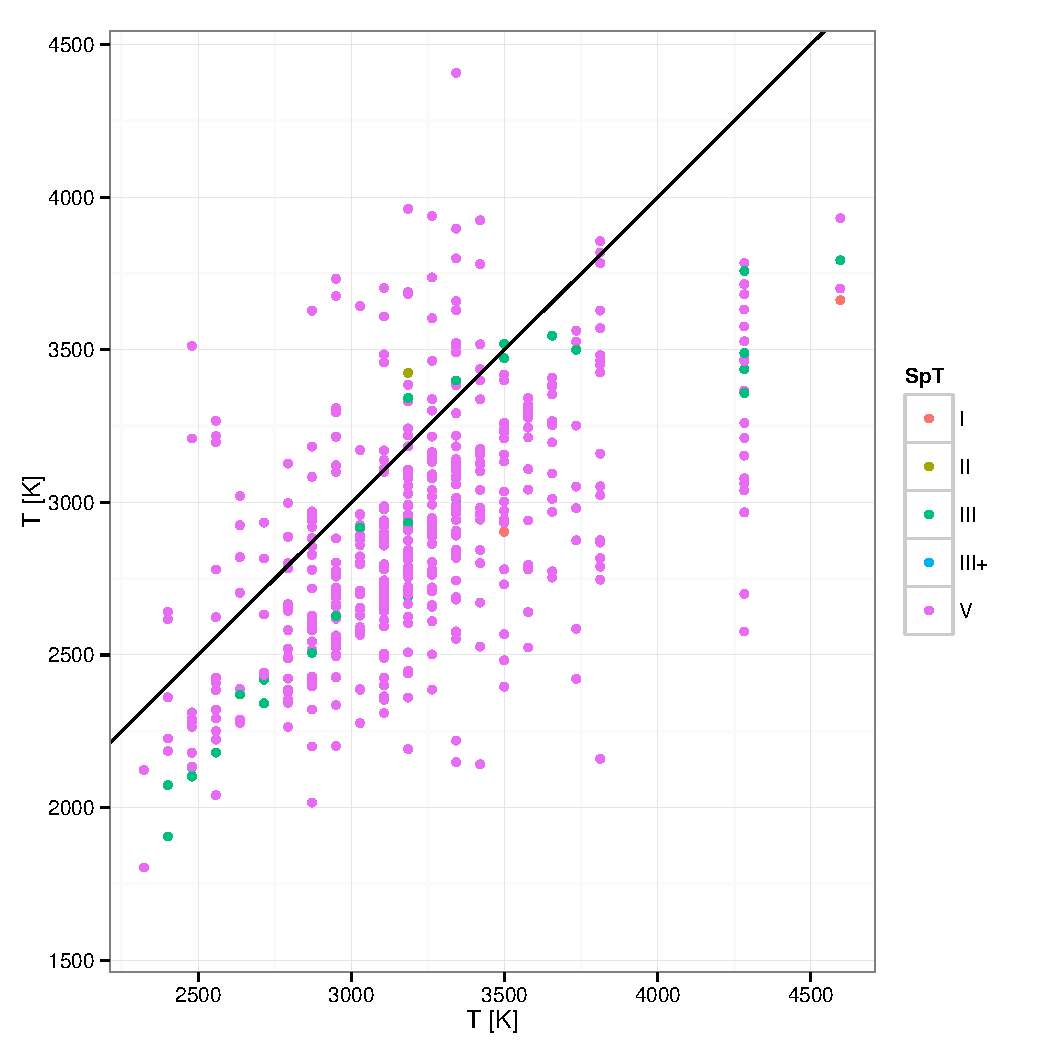
\includegraphics[width=6cm]{figs/T10BP_TSB.pdf}
 \caption{Comparison between Temperature estimations from Spectral Subtype 
 in x axis and the Random Forest for full length spectra trained with BT-Settl 
 at SNR=10 on y-axis}
 \label{fig:t10BP_tsb}
 \end{center}
\end {figure}

\begin {figure}
 \begin{center}
 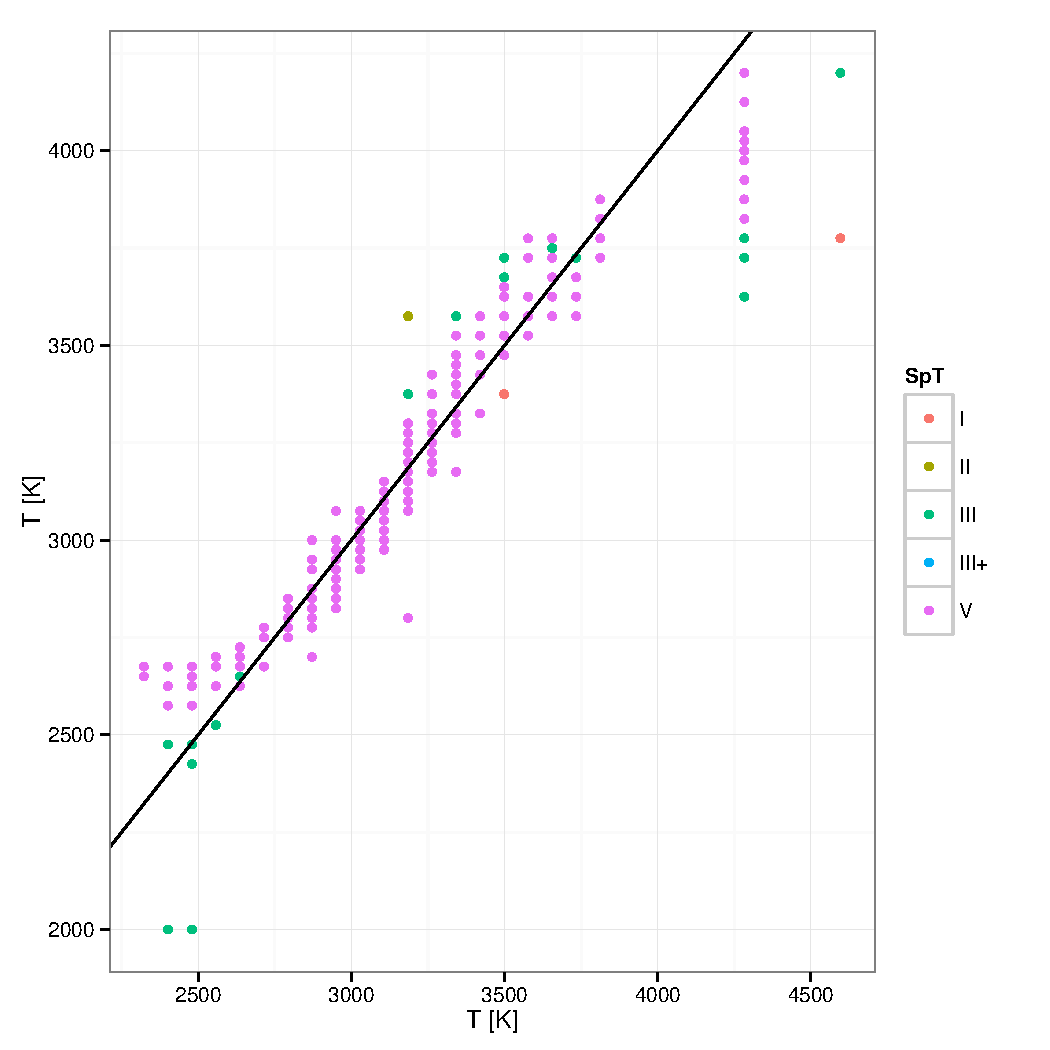
\includegraphics[width=6cm]{figs/T50CH_TSB.pdf}
 \caption{Comparison between Temperature estimations from Spectral Subtype 
 in x axis and the closest BT-Settl spectrum with SNR=50 on y-axis}
 \label{fig:t50bp_tsb}
 \end{center}
\end {figure}

\begin {figure}
 \begin{center}
 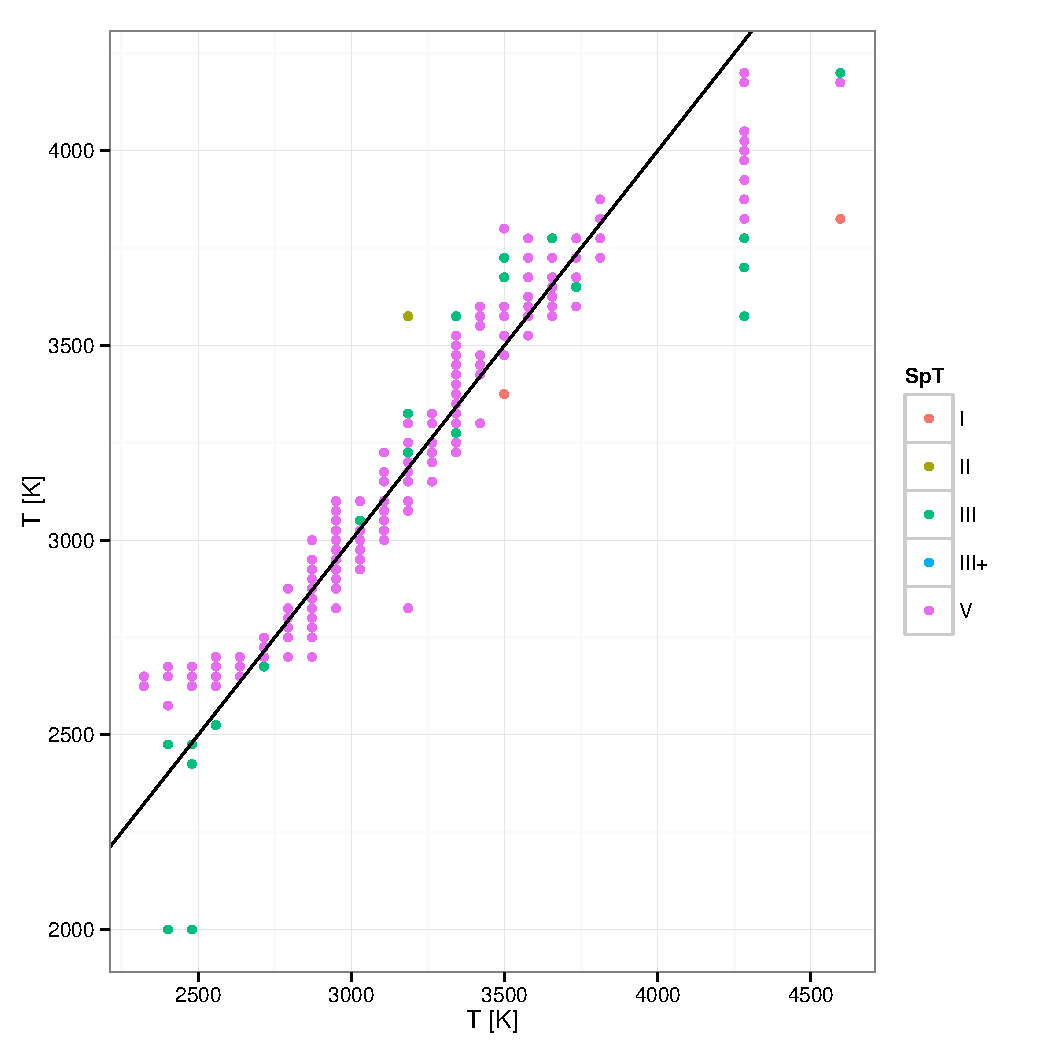
\includegraphics[width=6cm]{figs/T10CH_TSB.pdf}
 \caption{Comparison between Temperature estimations from Spectral Subtype 
 in x axis and the closest BT-Settl spectrum with SNR=10 on y-axis}
 \label{fig:t10BP_tsb}
 \end{center}
\end {figure}

% No le añado más discusión de momento, hasta ver si tiene sentido poer toda esta
% fila de gráficas o es mejor producir algo más condensado.
%
}


{
Te same approach can become useful to produce $log(gg)$ estimations. 
Here comparisons can only be possible between GA based features and
global spectra based approach.

In Figure~\ref{fig:Gbp_Gga_50} and Figure~\ref{fig:Gbp_Gga_10} 
relationships between $log(g)$ predicted by global espectrum estimation 
and GA feature based estimation can be observed.
Additionally Figure~\ref{fig:Gch_Gga_50} and Figure~\ref{fig:Gch_Gga_10}
present the relationship between the GA based estimation and the 
$\chi^2$ nearest BT-Settl spectrum.

\begin {figure}
 \begin{center}
 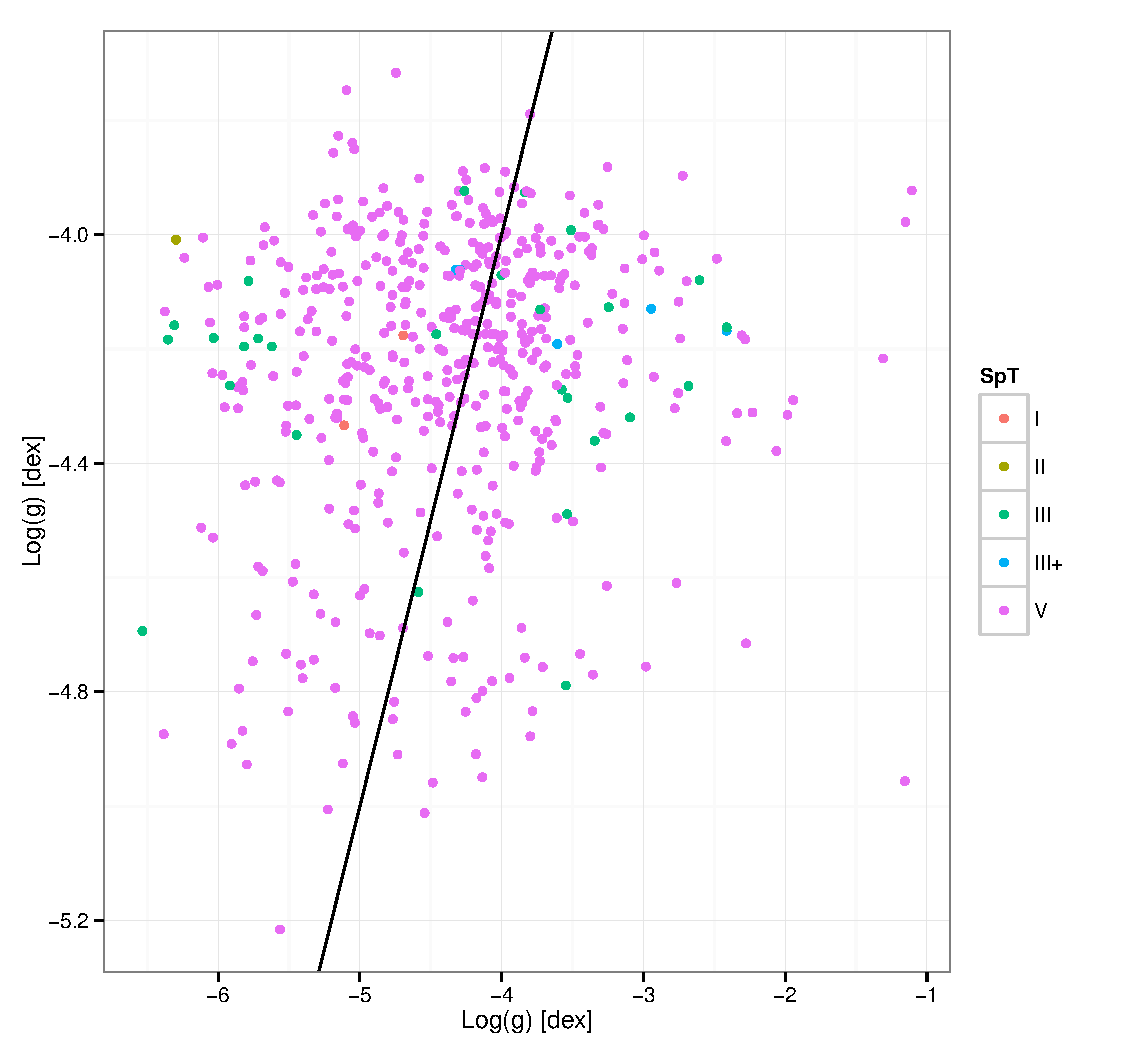
\includegraphics[width=6cm]{figs/LGBP_LGGA_50.pdf}
 \caption{Comparison between $log(g)$ estimations from 
 Random Forest model using GA features  in x axis and 
 the Global projected spectrum (ICA+SVM) with SNR=50 on y-axis}
 \label{fig:Gbp_Gga_50}
 \end{center}
\end {figure}

\begin {figure}
 \begin{center}
 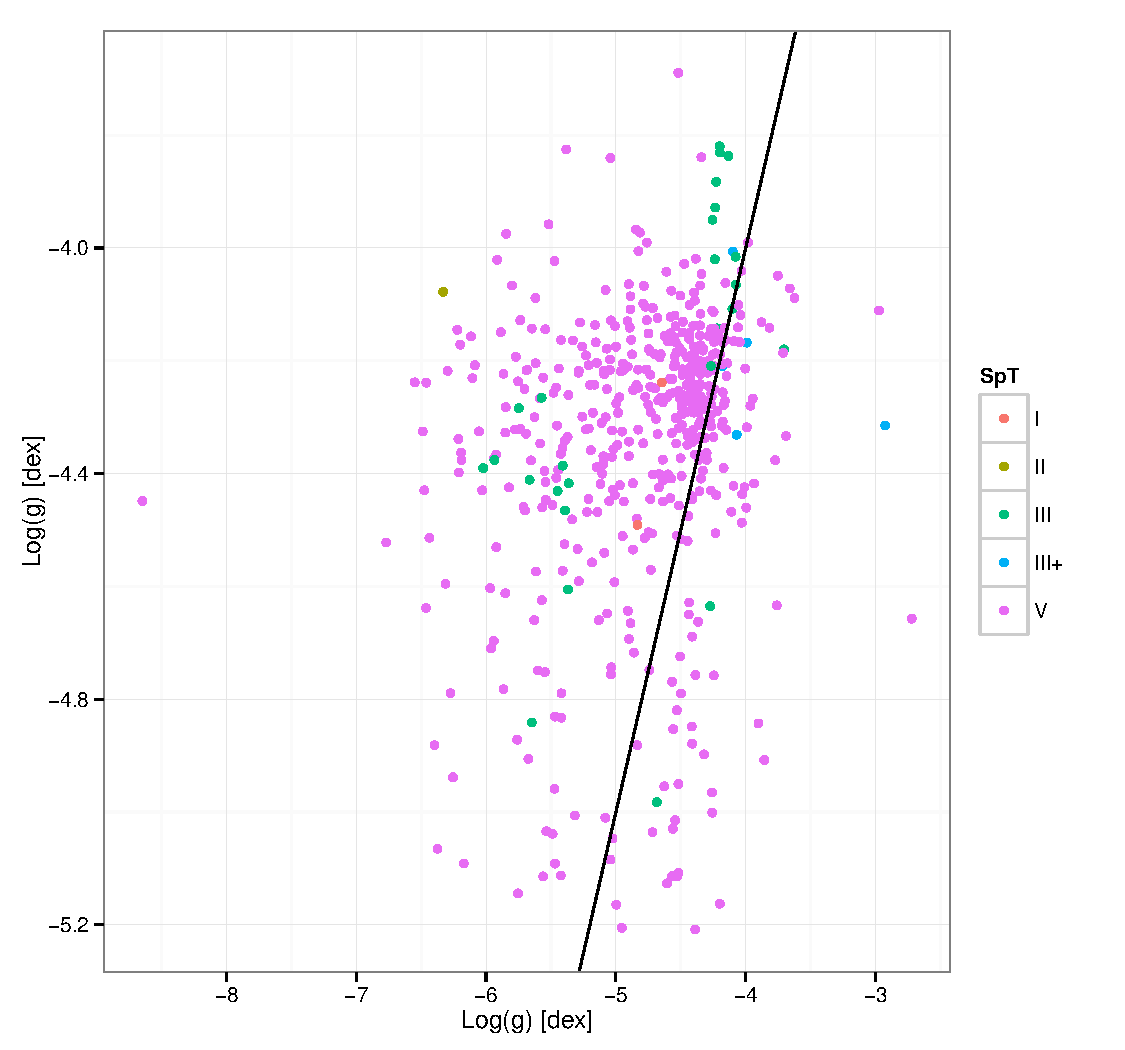
\includegraphics[width=6cm]{figs/LGBP_LGGA_10.pdf}
 \caption{Comparison between $log(g)$ estimations from 
 Random Forest model using GA features  in x axis and 
 the Global projected spectrum (ICA+SVM) with SNR=10 on y-axis}
 \label{fig:Gbp_Gga_10}
 \end{center}
\end {figure}

\begin {figure}
 \begin{center}
 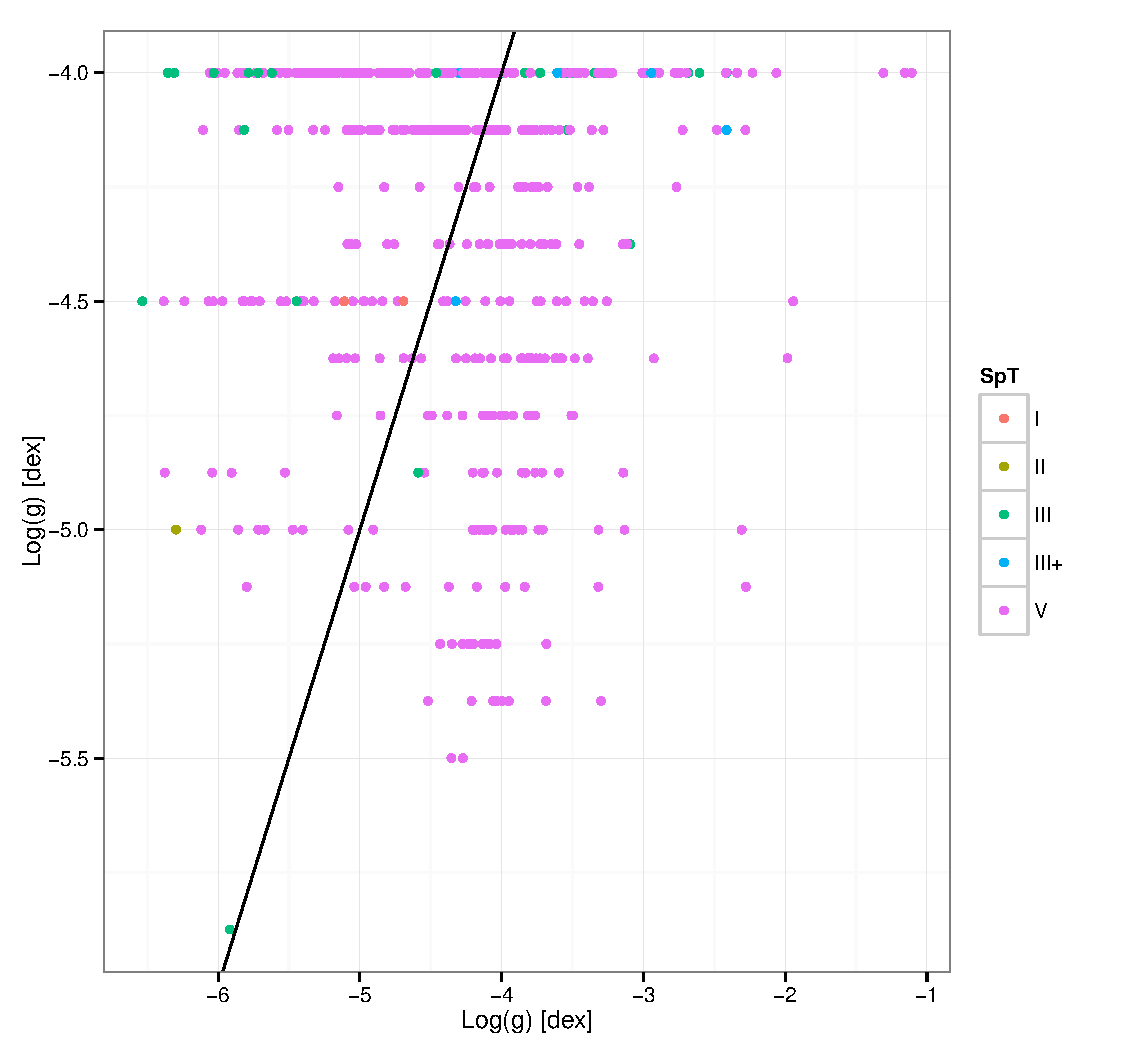
\includegraphics[width=6cm]{figs/LGCH_LGGA_50.pdf}
 \caption{Comparison between $log(g)$ estimations from 
 Random Forest model using GA features  in x axis and 
 the nearest $\chi^2$ BT-Settl spectrum with SNR=10 on y-axis}
 \label{fig:Gch_Gga_50}
 \end{center}
\end {figure}

\begin {figure}
 \begin{center}
 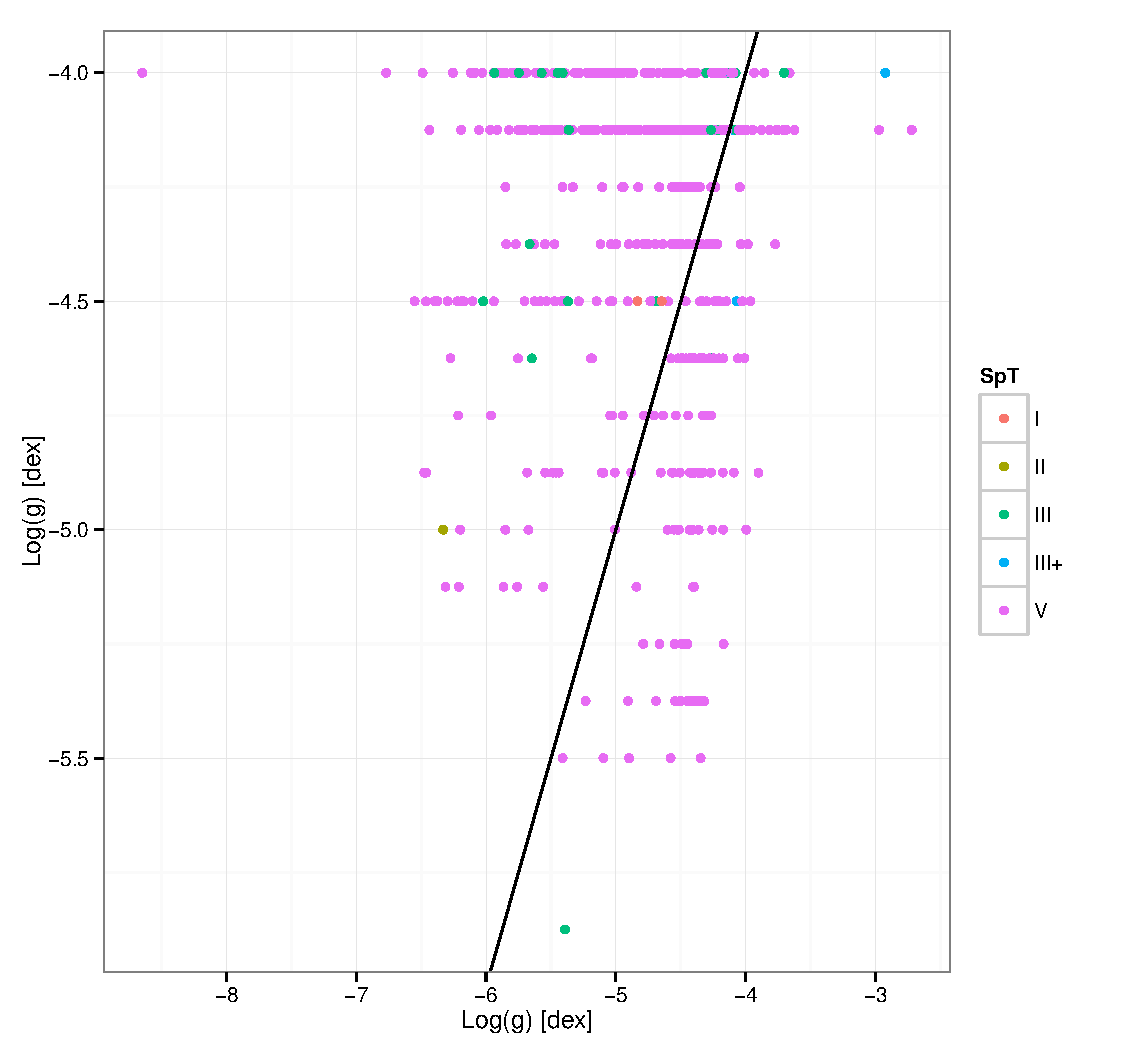
\includegraphics[width=6cm]{figs/LGCH_LGGA_10.pdf}
 \caption{Comparison between $log(g)$ estimations from 
 Random Forest model using GA features  in x axis and 
 the nearest $\chi^2$ BT-Settl spectrum with SNR=10 on y-axis}
 \label{fig:Gch_Gga_10}
 \end{center}
\end {figure}

% De nuevo las valoraciones deberían esperar a ver qué ponemos.

}

{ 

Finally, the same analysis is performed for the Metallicty parameter

\begin {figure}
 \begin{center}
 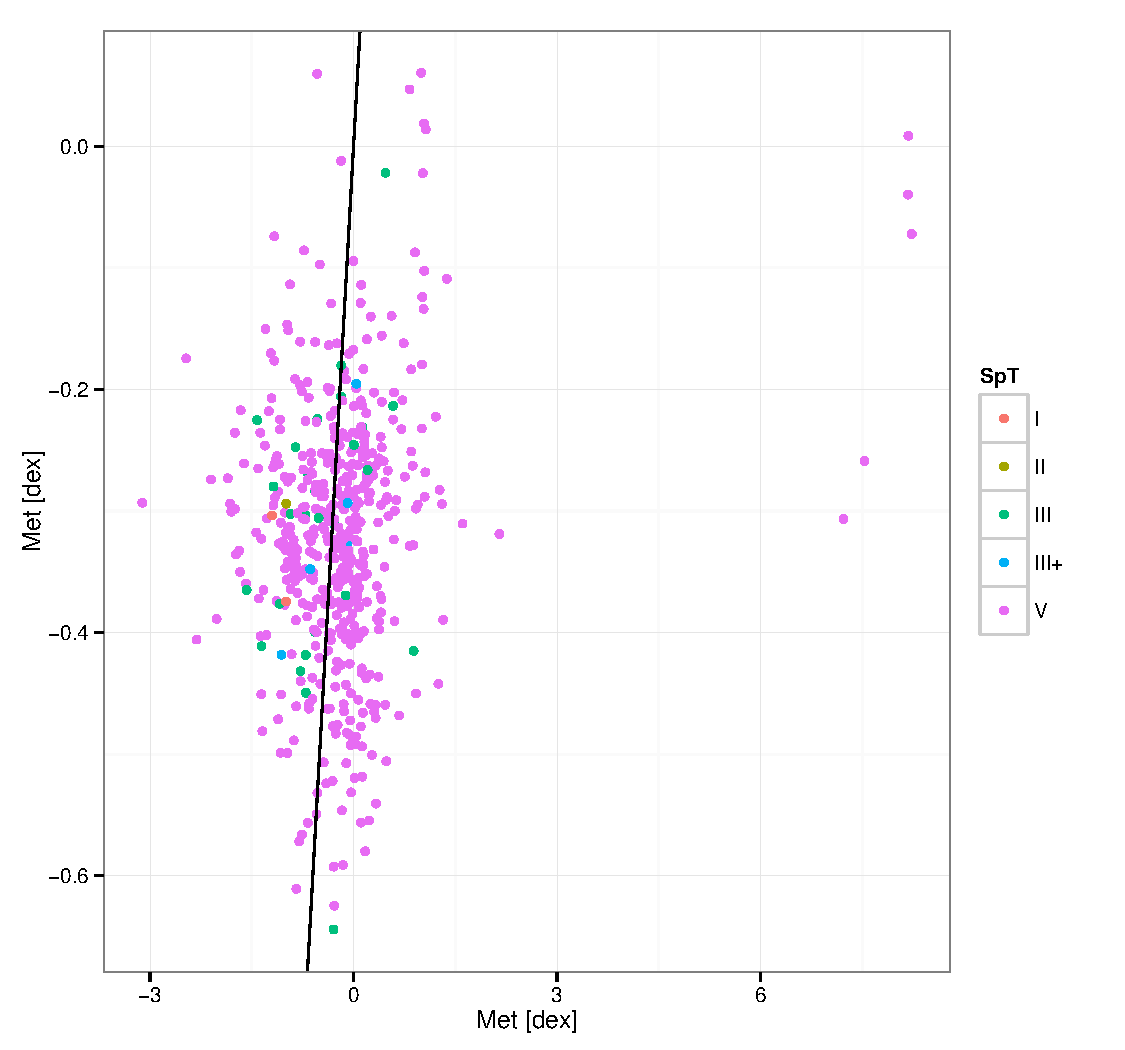
\includegraphics[width=6cm]{figs/MBP_MGA_50.pdf}
 \caption{Comparison between Metallicity estimations from 
 Random Forest model using GA features  in x axis and 
 the Global projected spectrum (ICA+SVM) with SNR=50 on y-axis}
 \label{fig:Mbp_Mga_50}
 \end{center}
\end {figure}

\begin {figure}
 \begin{center}
 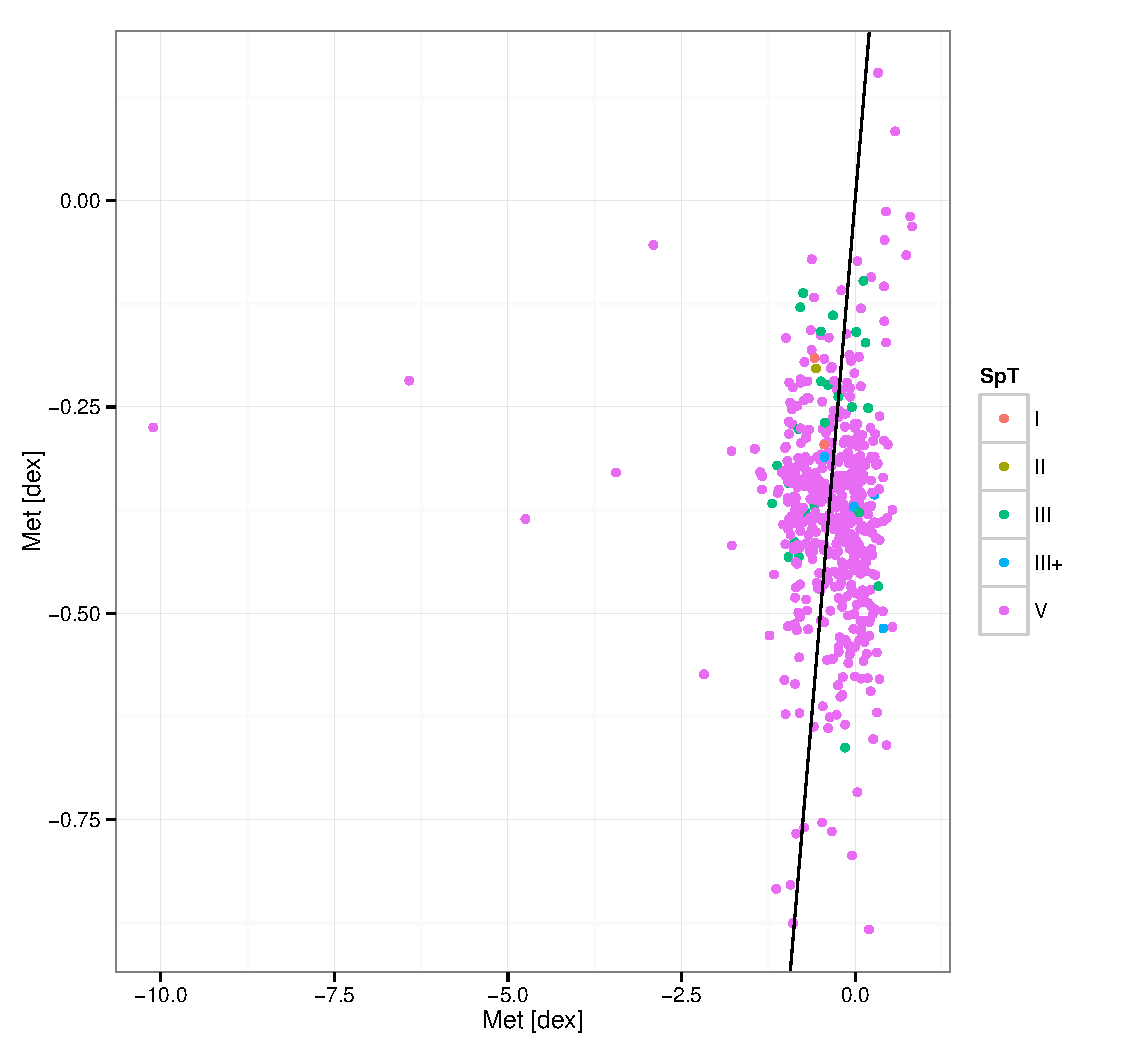
\includegraphics[width=6cm]{figs/MBP_MGA_10.pdf}
 \caption{Comparison between Metallicity estimations from 
 Random Forest model using GA features  in x axis and 
 the Global projected spectrum (ICA+SVM) with SNR=10 on y-axis}
 \label{fig:Mbp_Mga_10}
 \end{center}
\end {figure}

\begin {figure}
 \begin{center}
 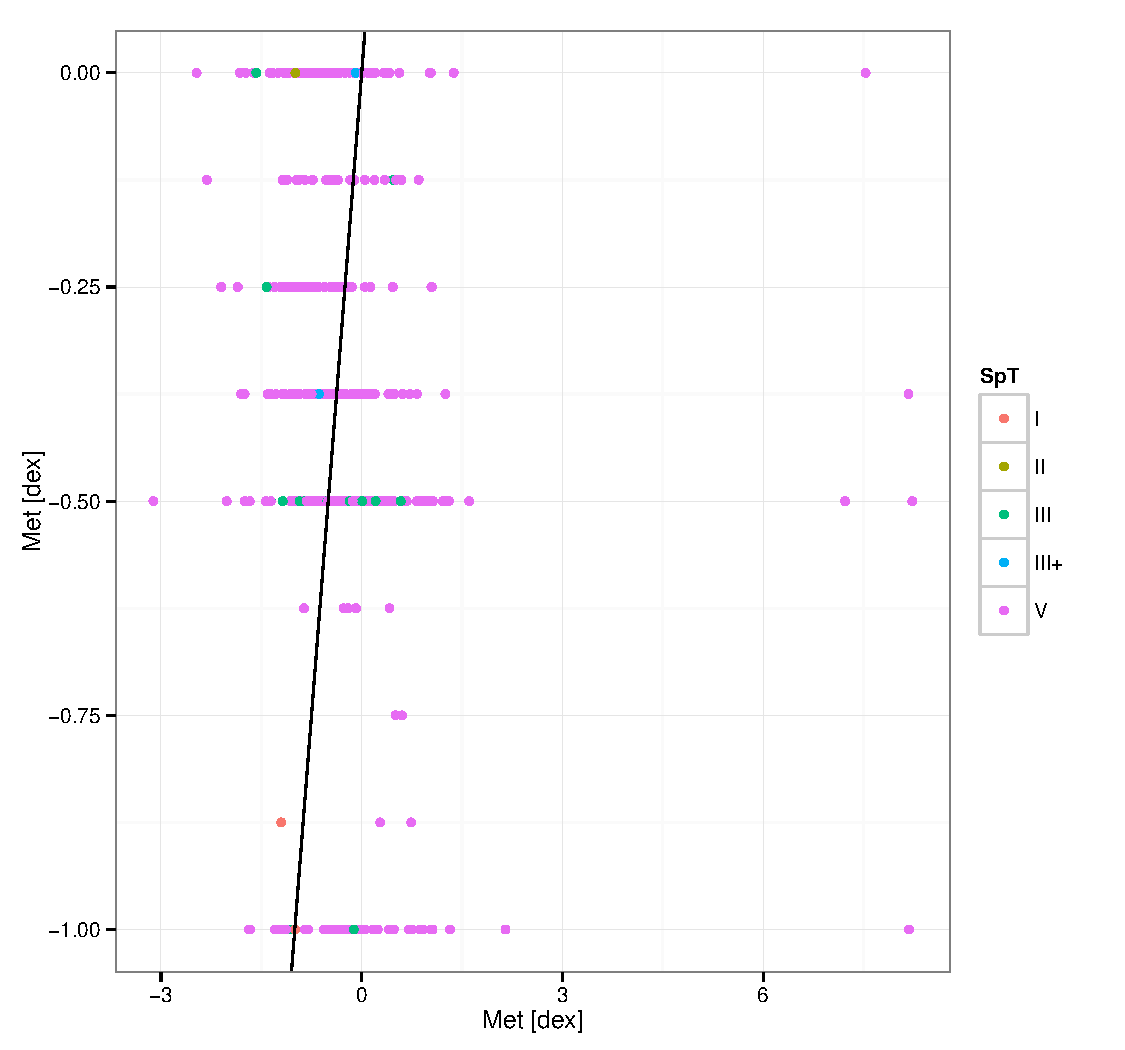
\includegraphics[width=6cm]{figs/MCH_MGA_50.pdf}
 \caption{Comparison between Metallicity estimations from 
 Random Forest model using GA features  in x axis and 
 the nearest $\chi^2$ BT-Settl spectrum with SNR=10 on y-axis}
 \label{fig:Mch_Mga_50}
 \end{center}
\end {figure}

\begin {figure}
 \begin{center}
 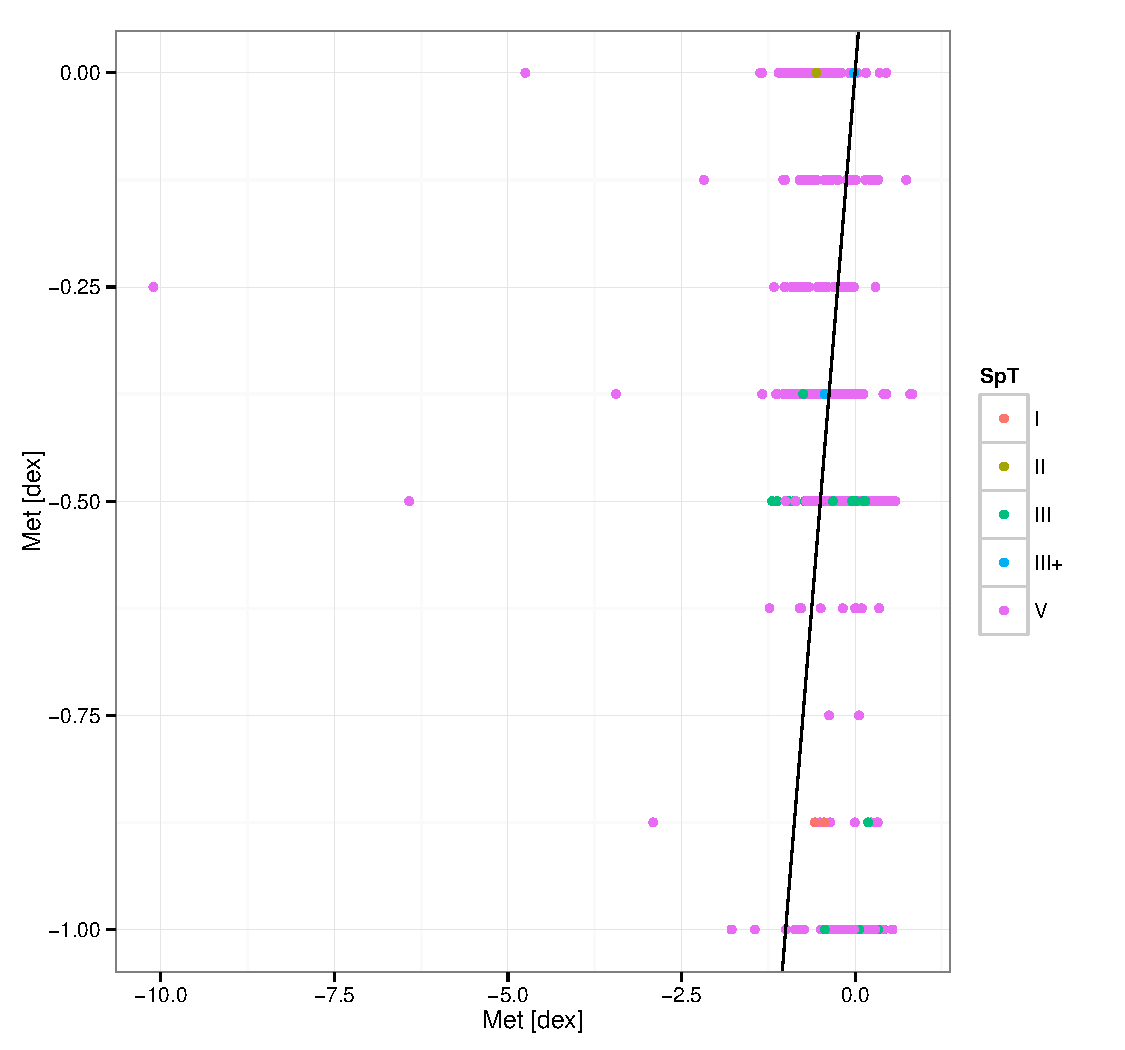
\includegraphics[width=6cm]{figs/MCH_MGA_10.pdf}
 \caption{Comparison between Metallicity estimations from 
 Random Forest model using GA features  in x axis and 
 the nearest $\chi^2$ BT-Settl spectrum with SNR=10 on y-axis}
 \label{fig:Mch_Mga_10}
 \end{center}
\end {figure}

% De nuevo, el análisis y discusión, función de lo que queramos dejar
}

{
It is possible to present relationships between $log(g)$ and $log(T_{eff})$
as a matter of congruence analysis between predictions.

\begin{figure}
 \begin{center}
 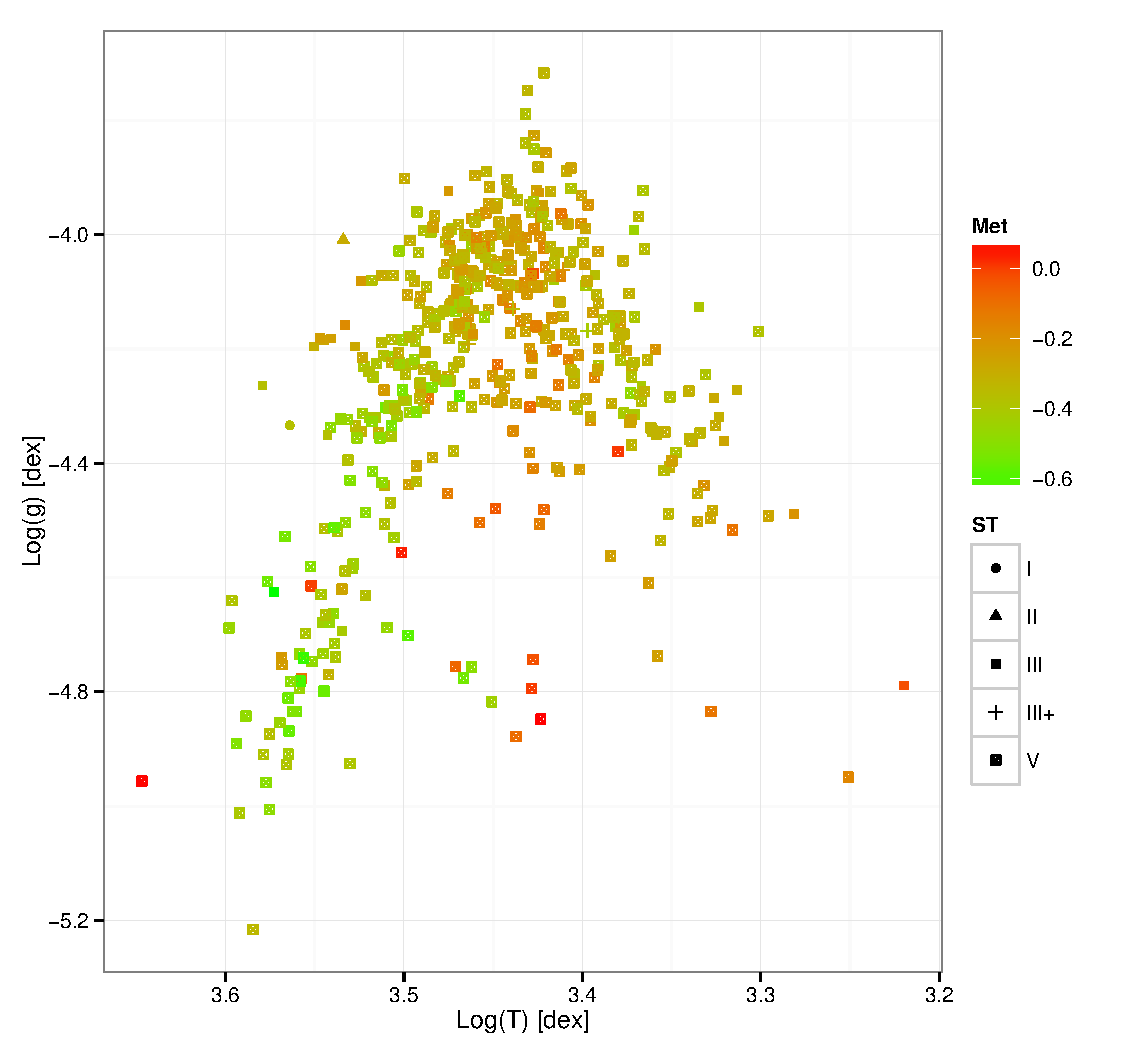
\includegraphics[width=6cm]{figs/LG_LT_BP_50.pdf}
 \caption{Relationship between $log(T_{eff}) $ in the x axis 
 and $log(g)$ in the y axis for SNR=50 when Global ICA+SVM model
 is used}
 \label{fig:lg_lt_bp_50}
 \end{center}
\end{figure}

\begin{figure} 
 \begin{center}
 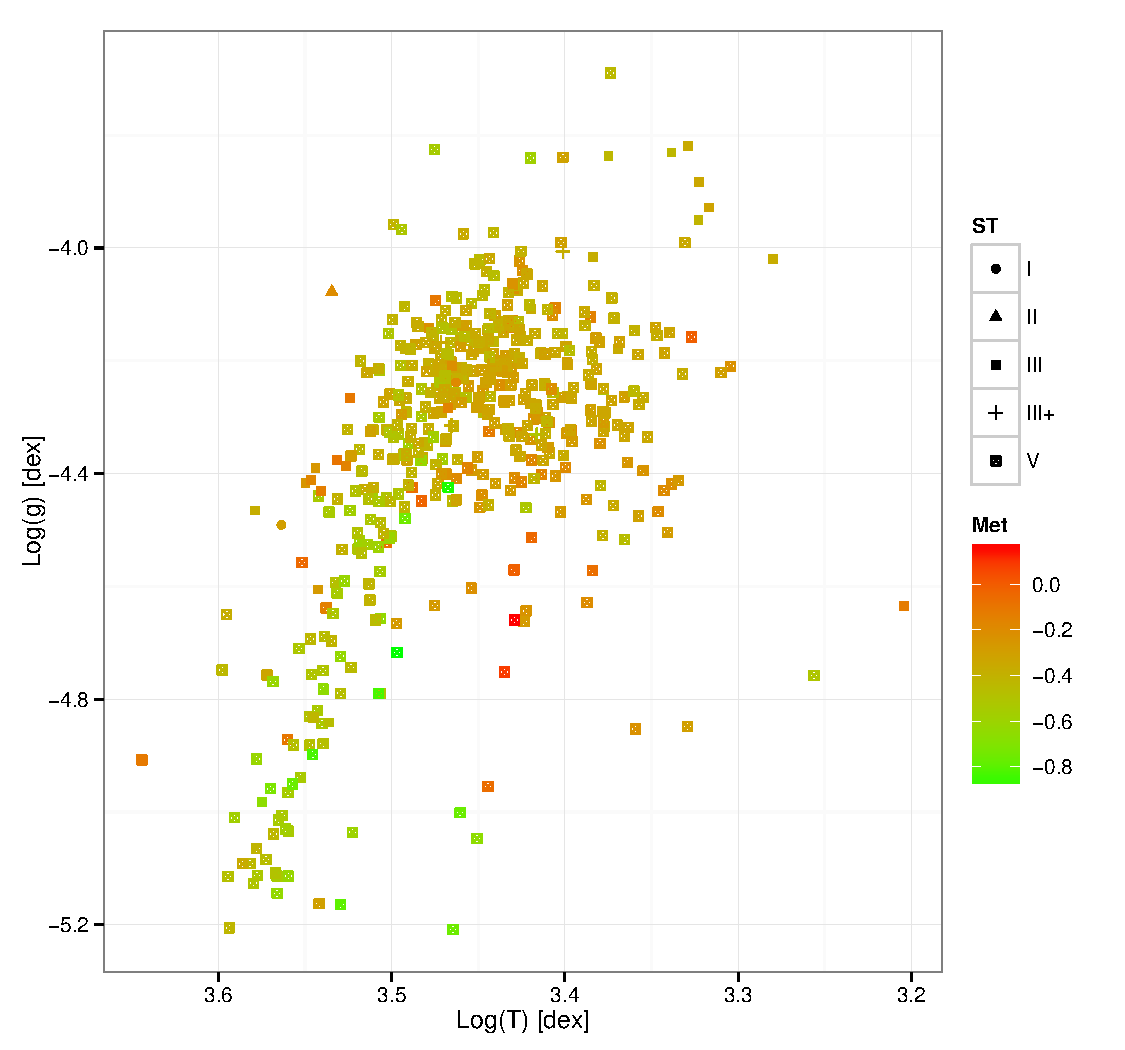
\includegraphics[width=6cm]{figs/LG_LT_BP_10.pdf}
 \caption{Relationship between $log(T_{eff}) $ in the x axis 
 and $log(g)$ in the y axis for SNR=10 when Global ICA+SVM model
 is used}
 \label{fig:lg_lt_bp_50}
 \end{center}
\end{figure}

The same can be performed when the estimations arise from models 
based on features provided by the GA technique.

\begin{figure}
 \begin{center}
 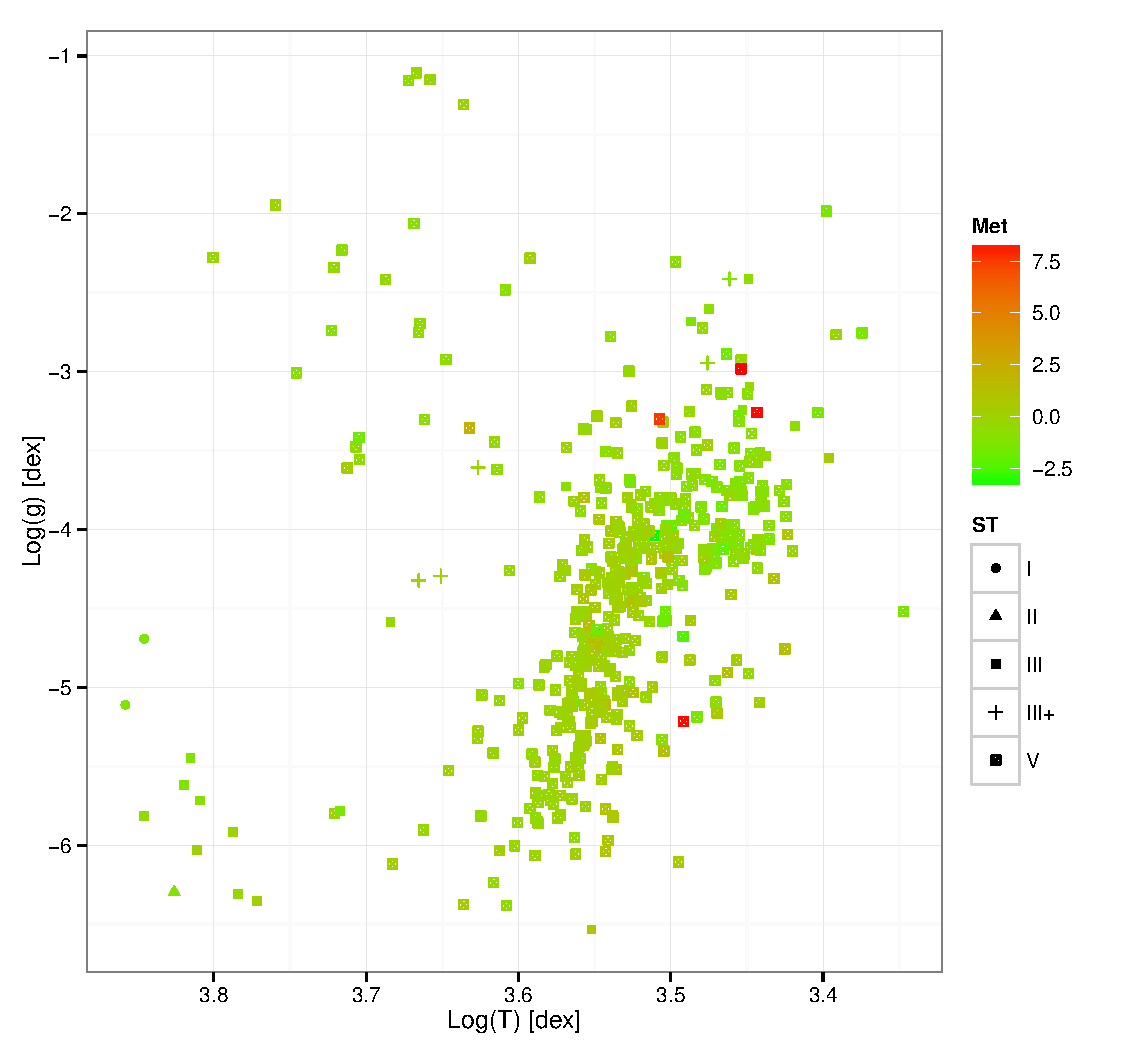
\includegraphics[width=6cm]{figs/LG_LT_GA_50.pdf}
 \caption{Relationship between $log(T_{eff}) $ in the x axis 
 and $log(g)$ in the y axis for SNR=50 when 
 the Random Forest model over the GA provided features 
 is used}
 \label{fig:lg_lt_ga_50}
 \end{center}
\end{figure}

\begin{figure}
 \begin{center}
 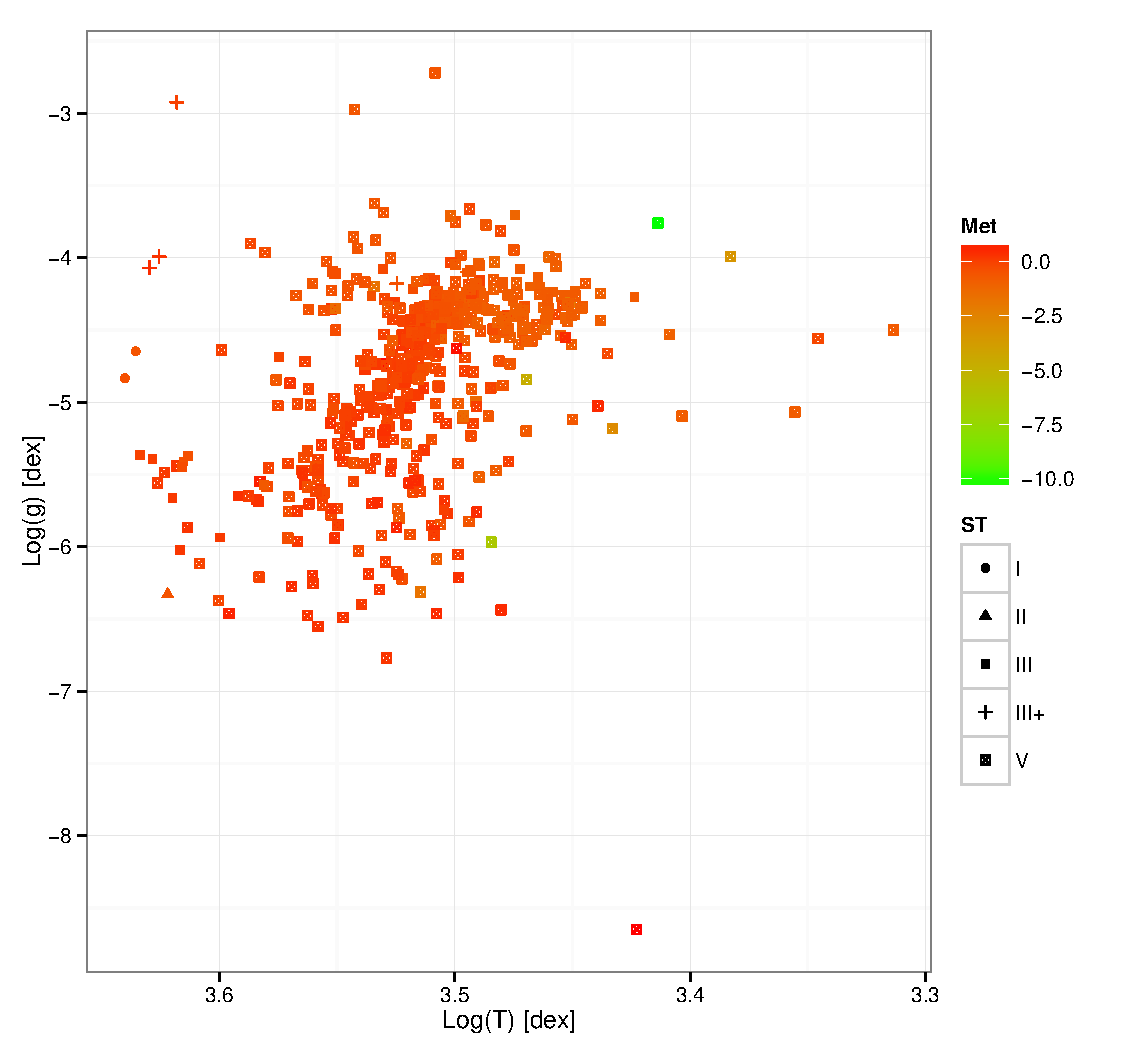
\includegraphics[width=6cm]{figs/LG_LT_GA_10.pdf}
 \caption{Relationship between $log(T_{eff}) $ in the x axis 
 and $log(g)$ in the y axis for SNR=10 when 
 the Random Forest model over the GA provided features 
 is used}
 \label{fig:lg_lt_ga_10}
 \end{center}
\end{figure}


And, for sure, it is possible to do it for estimations based on 
parameters from nearest labeled BT-Settl spectra.
In this particular case, it is possible to see how 
considering the global spectrum is positive for stronger 
physical parameters like $T_{eff}$ but the approach
reduces drastically its likelihood when other softer 
parameters are involved.

\clearpage 

\begin{figure}
 \begin{center}
 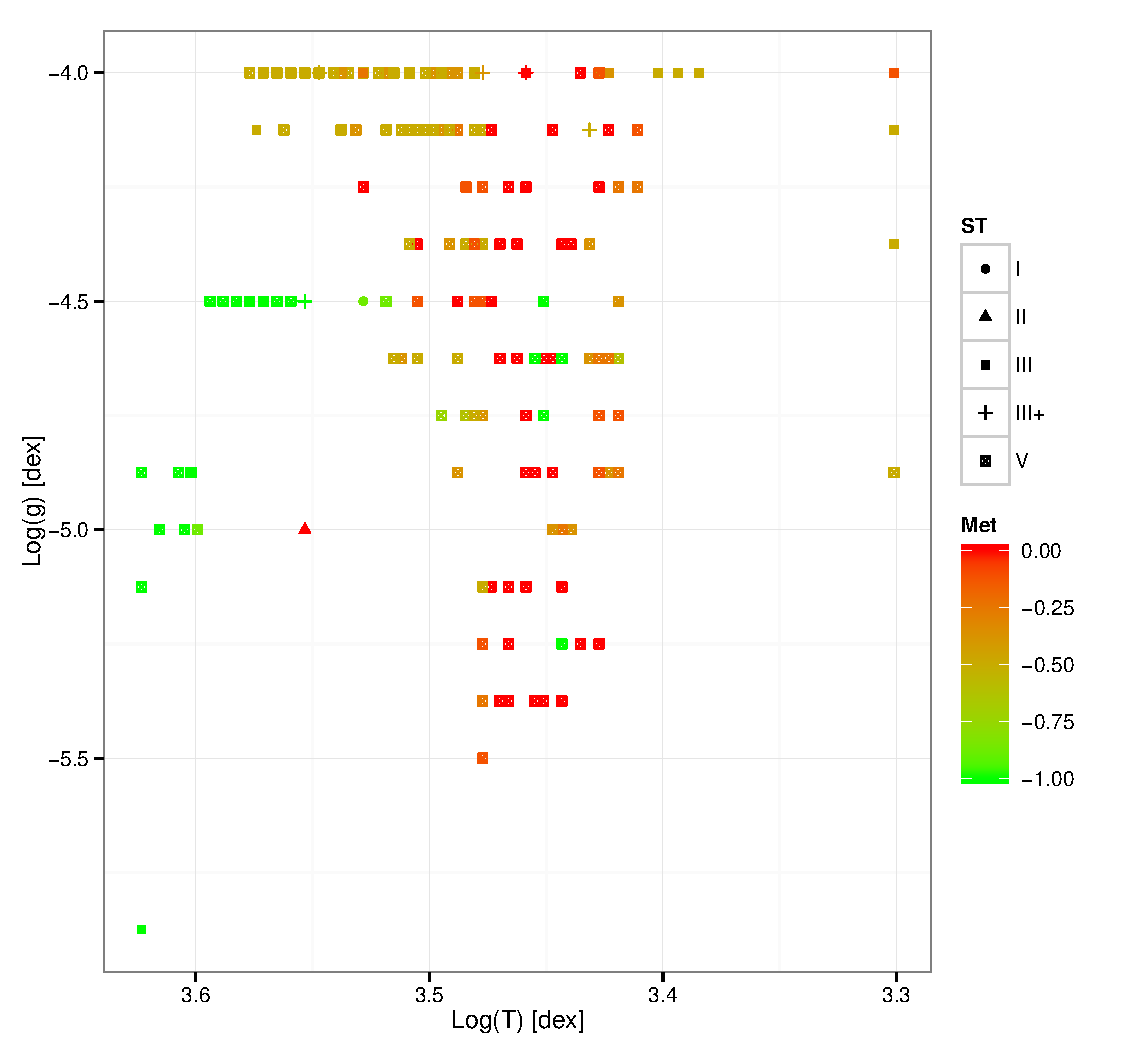
\includegraphics[width=6cm]{figs/LG_LT_CH_50.pdf}
 \caption{Relationship between $log(T_{eff}) $ in the x axis 
 and $log(g)$ in the y axis for SNR=50 when 
 the nearest BT-Settl spectrum is used}
 \label{fig:lg_lt_ch_50}
 \end{center}
\end{figure}

In the end deeper analysis needs to be carried out considering
several factors like coherence between labeled referenced 
library spectrum, density of the labeled spectra, etc.

\begin{figure}
 \begin{center}
 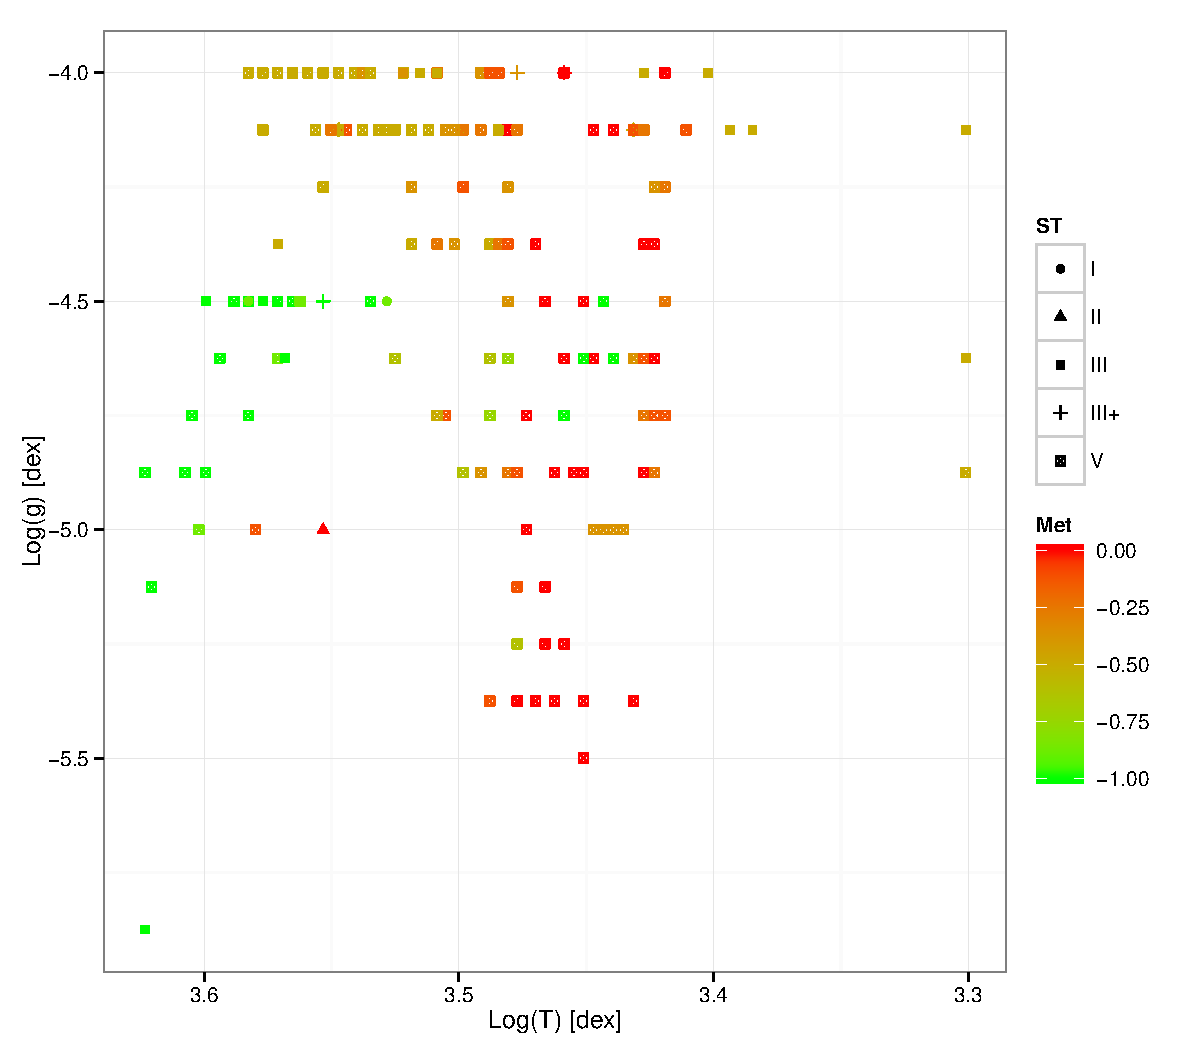
\includegraphics[width=6cm]{figs/LG_LT_CH_10.pdf}
 \caption{Relationship between $log(T_{eff}) $ in the x axis 
 and $log(g)$ in the y axis for SNR=10 when 
 the nearest BT-Settl spectrum is used}
 \label{fig:lg_lt_ch_10}
 \end{center}
\end{figure}


}